\newif\ifvimbug
\vimbugfalse

\ifvimbug
\begin{document}
	\fi
\exercise{Theoretical Questions}

\begin{questions}
%----------------------------------------------
\begin{question}{POMDP}{4}
	
		1) What is a POMDP? 
\begin{answer}
	
	POMDP stands for \textit{Partial Observable Markov Decision Proces}. In such a Process the real state can not be obtained by the agent but an observation and it's confidence. [c.f. 08-PoMDPs p. 4]
\end{answer}

	2) How is it defined? (formal) 
\begin{answer}
	
	A POMDP is defined by:
	\begin{enumerate}
		\item its state space $s \in S$
		\item its action space $a \in A$
		\item its observation space $ o \in O$
		\item its transition dynamics $ \Pr(s'|s,a) = P_{s's}^a$
		\item its observation probabilities $O(o|s) = O_{os}$
		\item its reward function $r(s,a) = R_s^a$
		\item its initial state probabilities $\mu_0(s)$
		\item the history $h_t = (o_1, a_1 ,...,a_{t-1}, o_t)$, that contains all past states and actions
	\end{enumerate}
	[from 08-PoMDPs p. 5]
\end{answer}

	3) How is it different from a common MDP? 
\begin{answer}
	
	The \textbf{true state} is hidden. Thus the agents have to work with observations. For that, all the history of the actions and observations of all the agents have to be saved. (To make assumptions on the real state and thus the expected reward.)
\end{answer}

	4) 		Given an example of a POMDP
\begin{answer}
	
	A typical example for this problem is the \textit{tiger-door problem}.
	The agent can choose to open one of two doors, behind one of them is a reward and one the other contains punishment. However the agent can only observe the the true state with a probability distribution, through listening.
	[c.f. 08-PoMDPs p. 7]
\end{answer}
\end{question}



\begin{question}{State Definitions}{3}
	
	1) Name the different state definitions, introduced in the lecture.
\begin{answer}
	
	\begin{enumerate}
		\item Information state
		\item Belief state
	\end{enumerate}

\end{answer}
	
	2) How do they differ from one another?
\begin{answer}
	
	The \textit{information state} contains the whole history of actions and observations.
	The \textit{belief state} describes a probability distribution over states, given the past observations.
\end{answer}
	
	3) What are their advantages/disadvantages?
\begin{answer}
	
	The \textit{information state} allows for explicit evaluation for each time step. But is grows exponentially in the amount of steps ($T$).
	The \textit{belief state} is a possibly much shorter description of the \textit{true state}. For discrete states: In order to compute the Bellman equation we need to discretize the belief state.
\end{answer}
[c.f. from 08-PoMDPs pp. 10 ff.]
\end{question}


\begin{question}{Alpha Vectors}{3}
	
	1) What are alpha vectors?
	2) How do they relate to POMDPs?
	\begin{answer}
		
		One alpha vectors represent the reward from the value function over the state space for one action.
		The set of alpha vectors that lie on the upper convex hull represent the best possible actions under the current belief state.
		[c.f. from 08-PoMDPs pp. 24-26]
	\end{answer}
	
	3) Which property allows us to use them?
	\begin{answer}
		
		The reward function of the Bellman equation for the value Iteration is linear in the belief state $b$ ($b: p(b,a) = \sum_s b(s)r(s,a)$). The max-pooling over all actions implies a piecewise linearity in $b$ for $V^*(b)$ (convexity).
	\end{answer}
\end{question}


\begin{question}{Belief-State Value Iteration}{4}
	
	1) Describe Belief-State Value Iteration
	\begin{answer}
		
		We iterate over the most probable action-observations transitions to obtain the maximal reward in the previous step. This results in the state, we belief to have obtained for the chosen action.
		%todo: check whether this holds, or even if this is understandable in the first place
	\end{answer}
	
	2) How are alpha vectors used?
	\begin{answer}
		
		An alpha vector is used to compute the reward function of an belief state for a policy tree.
		[c.f. 08-PoMDPs p.28]
	\end{answer}
	
	3) What are the main update steps?
	\begin{answer}
		
		There are three update steps:
		\begin{enumerate}
			\item Get the $\max_\alpha (s)$ for the action space and the possible thereafter observations $o'$
			\item Averaging over the observations $o'$ and adding reward leads to the optimal Q values $Q_{t-1}^*$
			\item Consider the best actions ($\max_\alpha b$) to obtain $V_{t-1}^*$
		\end{enumerate}
		[c.f. 08-PoMDPs pp. 29-30]
	\end{answer}
\end{question}


\begin{question}{Point-Based Value Iteration}{4}
	
	1) Describe Point-Based Value Iteration
	\begin{answer}
		
		Same as the Belief-State Value Iteration, but only rely on a small set of belief states.
		Updates the belief state in polynomial time. 
	\end{answer}
	
	2) How are alpha vectors used?
	\begin{answer}
		
		Each alpha vectors represent a \textit{reward "function"} for the state space.
	\end{answer}
	
	3) What are the main update steps?
	\begin{answer}
		
		\begin{enumerate}
		\item "Compute alpha vectors for actions and observations"
		\item For a subset of belief states, "average over observations, add reward".
		\item "Find best action for each belief point."
		\end{enumerate}
		[c.f. 08-PoMDPs p. 34]
	\end{answer}
\end{question}


\begin{question}{Bayes Adaptive MDPs}{4}
	
	1) What is the main concept of BAMDPs? When are they useful?
	\begin{answer}
		
		"A Bayes Adaptive MDP defines a POMDP with the MDP model as unobserved state".
		We put a posterior in the state space. 
		The agent is aware and can define any uncertainty in its partial observed model.
		[c.f. 08-PoMDPs p. 76]
	\end{answer}
	
	2) Why is a Dirichlet distribution a good prior for discrete systems?
	\begin{answer}
		
		"[T]he Dirichlet distribution is the conjugate prior of the categorical distribution and multinomial distribution."
		[c.f. https://en.wikipedia.org/wiki/Dirichlet\_distribution]
		Which fits to our case if the set of states $S$ and set of actions $A$ are discrete (nominal).
	\end{answer}
	
		3) When does a BAMDP become a BAPOMDP?
	\begin{answer}
		
		BAMDPs become BAPOMDPs, when we can measure the true states $s$ and $s'$, but only an observation model $O_{os} = p(o|s)$.
		[c.f. 08-PoMDPs p. 79]
	\end{answer}
	
		4) Can we use Belief-State Value Iteration on BAPOMDPs? Is it a good idea?
		\begin{answer}
			
			The belief state easily becomes huge, as we have to consider the transition history. This makes the Belief-State Value Iteration on BAPOMDPs feasible, only for small problems.
			[c.f. 08-PoMDPs pp. 79-80]
		\end{answer}
\end{question}


\begin{question}{Decentralized POMDPs}{4}
	
	1) How do they differ from common to POMDPs??
	\begin{answer}
		
		POMDPs consider problems, or more specific the view on the problem in the perspective of a single agent.
		Decentralized POMDPs, consider partial observable from a point of view with multiple agents.
		[c.f. 09-DecPoMDPs p. 1]
	\end{answer}
	
	2) How is a Dec-POMDP defined? (formal)
	\begin{answer}
		
		A Dec-POMDP is defined by:
		\begin{enumerate}
			\item it's state space $ s \in S$
			\item an action space $A_i$ for each agent $i$
			\item an observation space $O_i$ for each agent $i$
			\item the state-action transition dynamics $P(s'|s,a) = P_{s' s}^a$
			\item an observation model per agent $i$ : $O_i(o|s) = O_{o s}^i$
			\item a shared reward function for all agents $I$: $r(s,a) = R_s^a$
			\item the initial state probabilities $\mu_0(s)$.
		\end{enumerate}
		[c.f. 09-DecPoMDPs p. 4]
	\end{answer}
	
	3) Can we use the same algorithms as for common POMDPs? Why?
	\begin{answer}
		
		We can not use the PoMDP algorithm directly. 
		The state representation of each agent now not only consists of it's on observation history, but every possible other agents observation history as well.
		A \textit{local policy} is map from an observation history $o^i = (o_1^i, ..., o_t^i)$ to actions.
		Since each agent can only observe the other actions with some certainty, each agent $i$ have to save a set of possible local policies $\Pi_i$ for each other agent $\not \in i$. The set of polices for each other agent is denoted as \textit{joint policy} $\langle \pi_1, ..., \pi_n \rangle$.
		[c.f. 09-DecPoMDPs p. 7 and 9]
		In order to solve a Dec-POMDP we can now perform an exhaustive search over the piecewise product of combinations of the set of joint policies to find the optimal set of local policies.
		[c.f. 09-DecPoMDPs pp.12 ff.]
	\end{answer}
	
	4) Are there other ways to solve Dec-POMDPs? Explain one conceptually
	\begin{answer}
		
		The \textit{joint policy} may be represented as a set of trees.
		The root and the nodes (as well as the leafs) are the actions, which are connected via the observations (edges).
		We can evaluate the values of each tree.
		[c.f. 09-DecPoMDPs pp. 7 and 12]
		Since there will be many trees that do not contribute to the optimal solutions, we can prune (exclude) these trees.
		[c.f. 09-DecPoMDPs p. 16]
		"We  can prune a tree $q_i$ if there is a distribution $x(q_i^{-1})$ of other trees that has a higher value for all system states and trees of the other agent."
		[09-DecPoMDPs p. 18]
	\end{answer}
	\newpage
	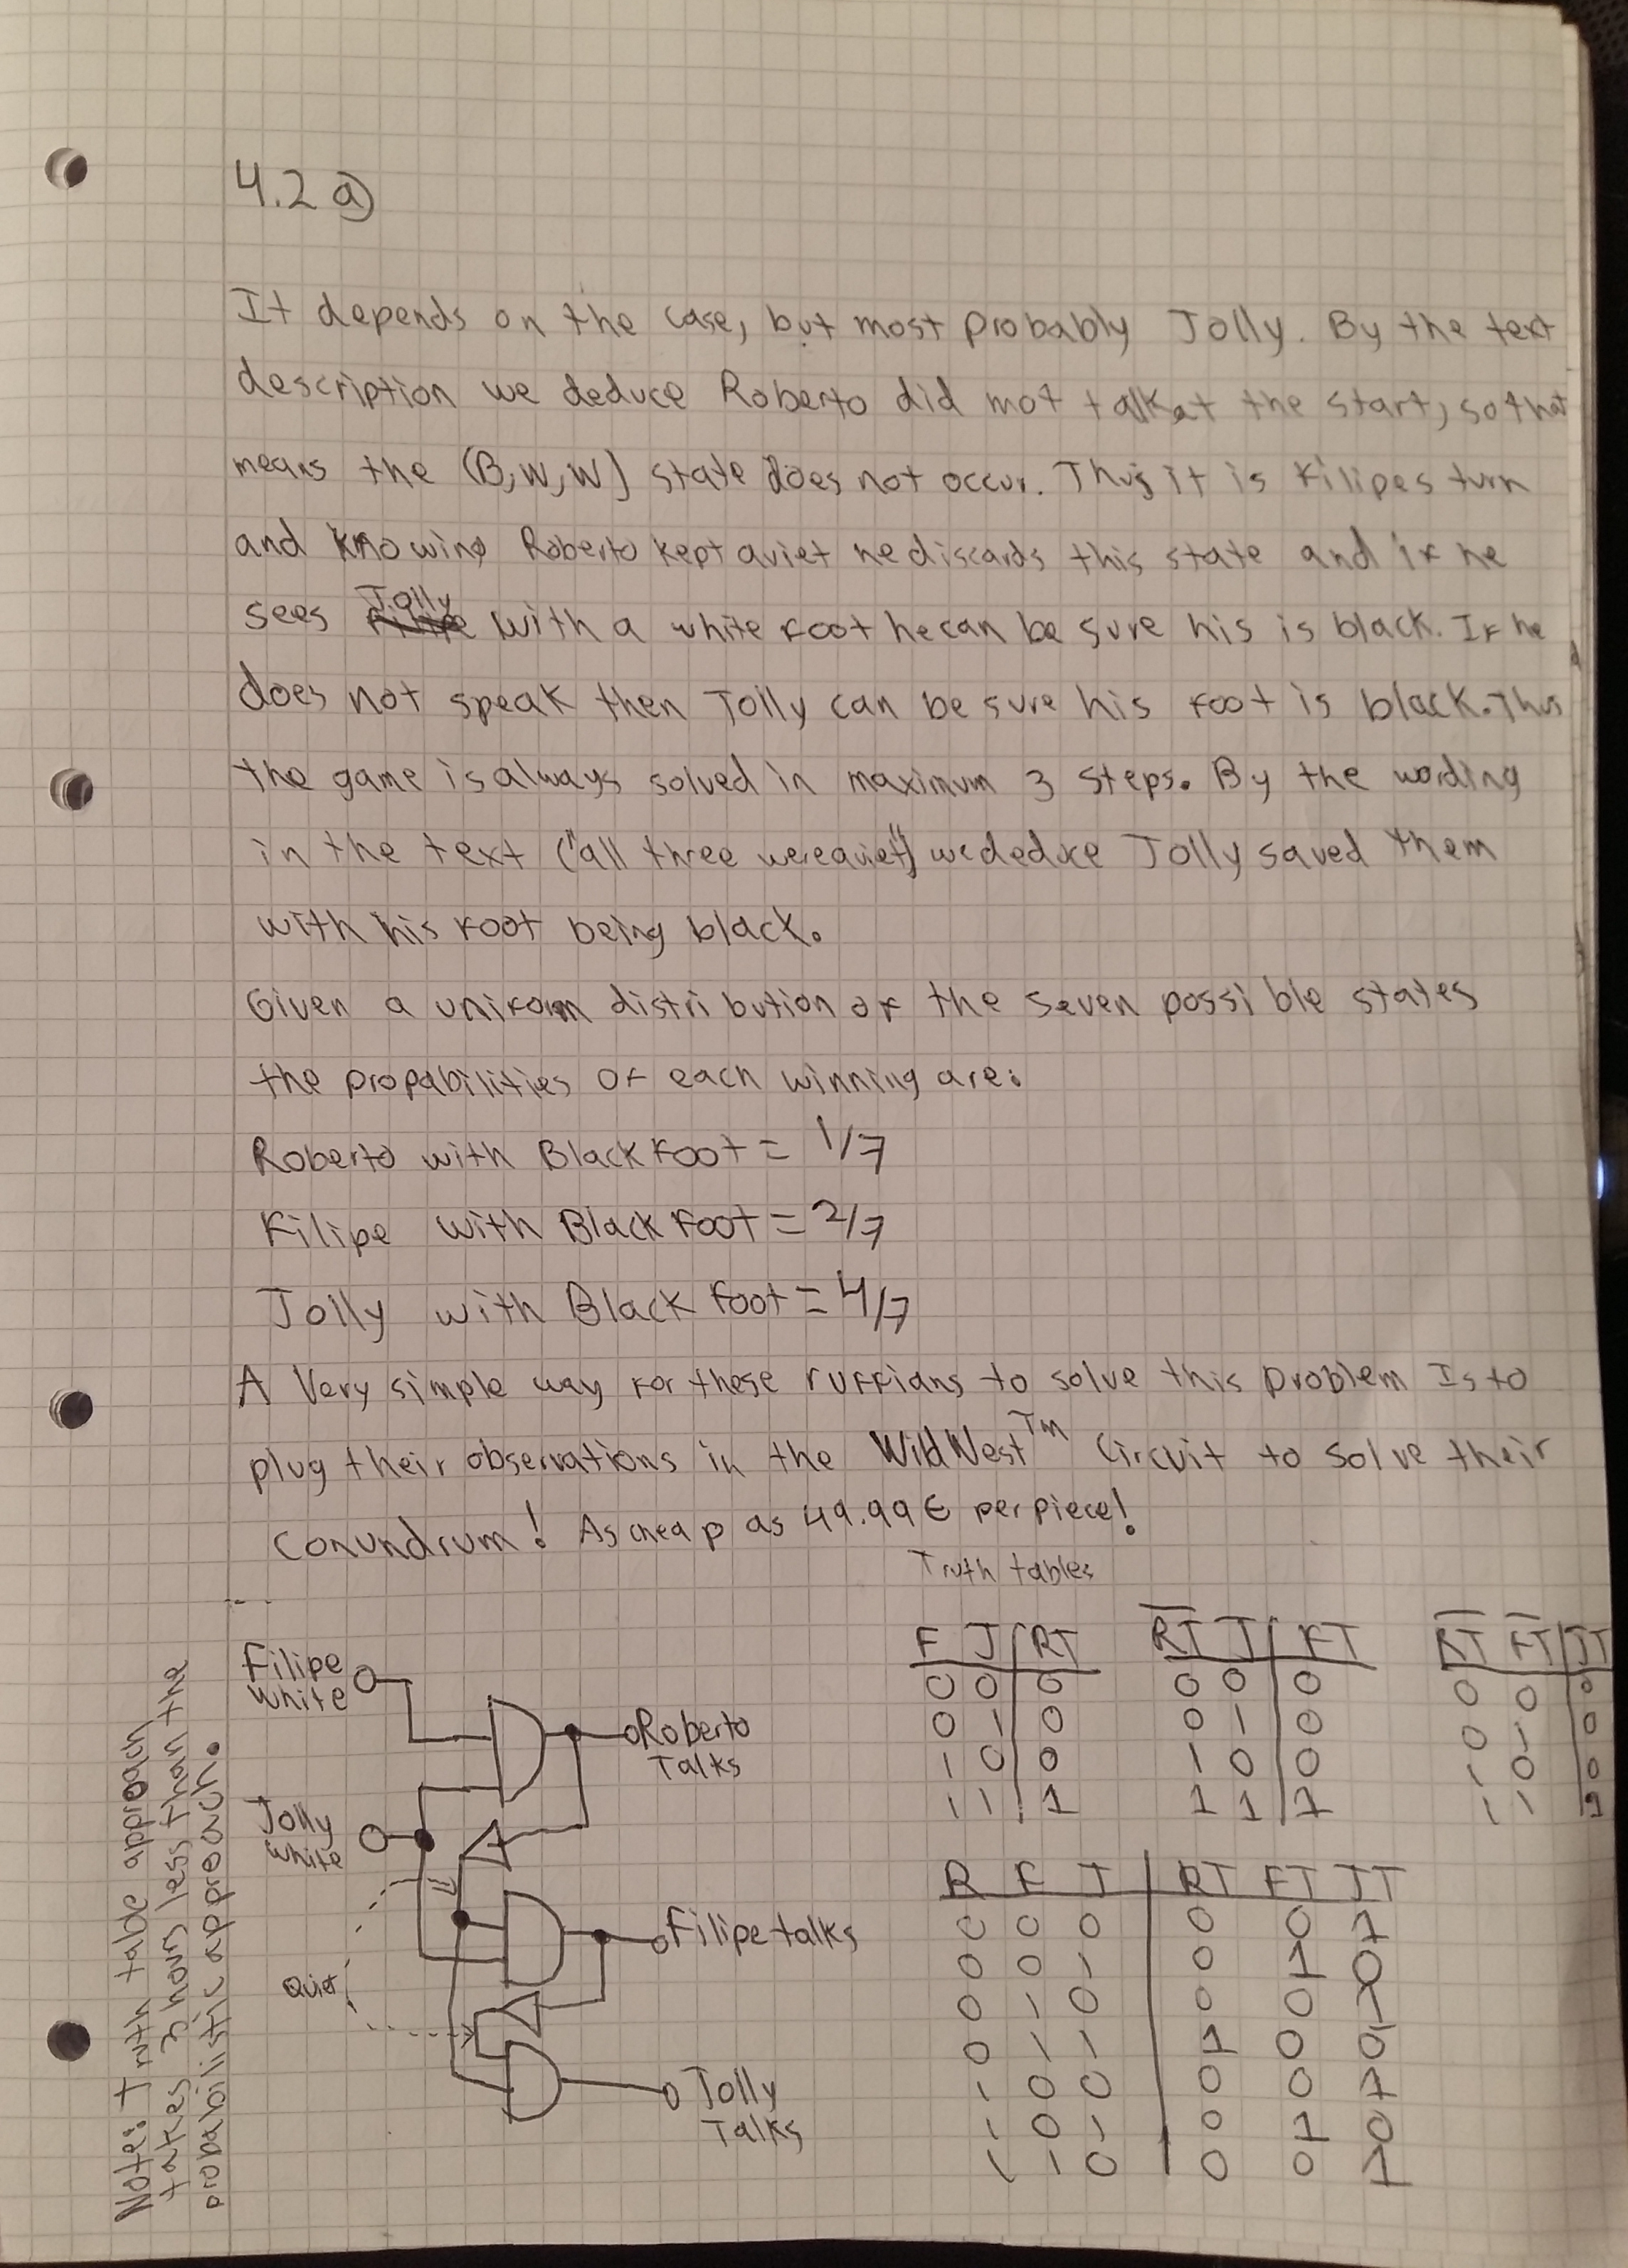
\includegraphics[scale=0.2]{p1.jpg}
	\newpage
	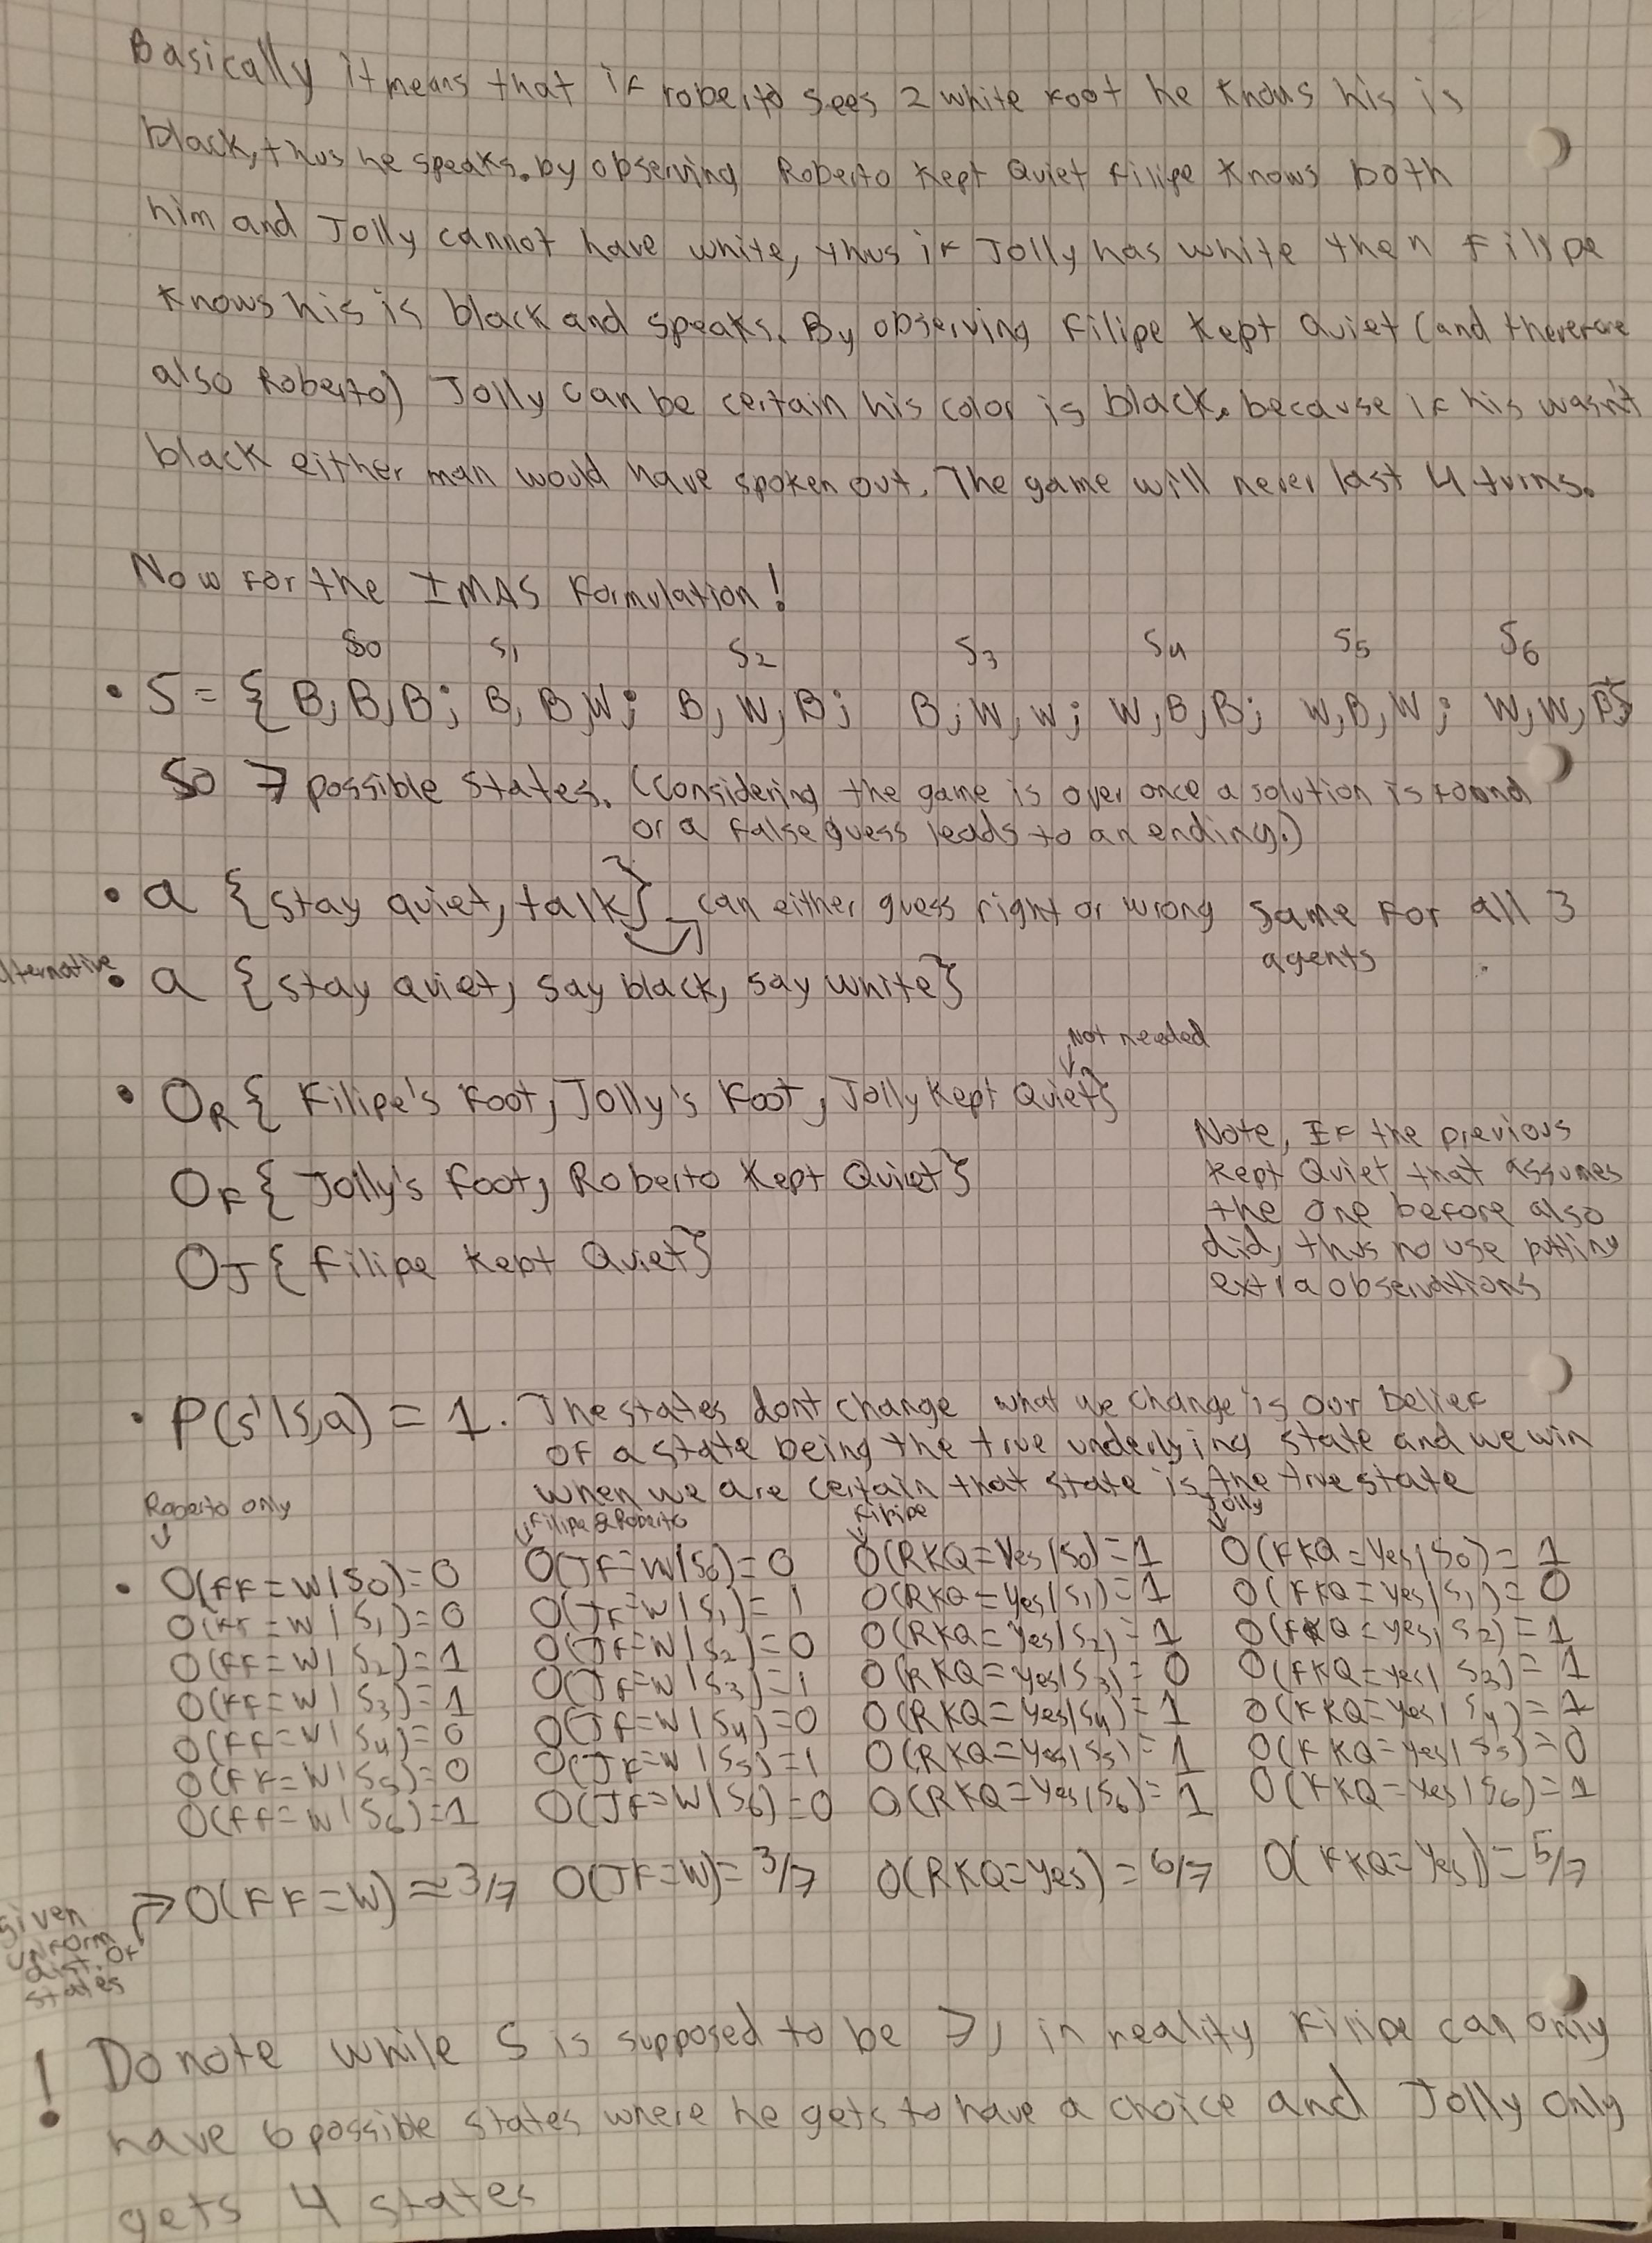
\includegraphics[scale=0.2]{p2.jpg}
		\newpage

	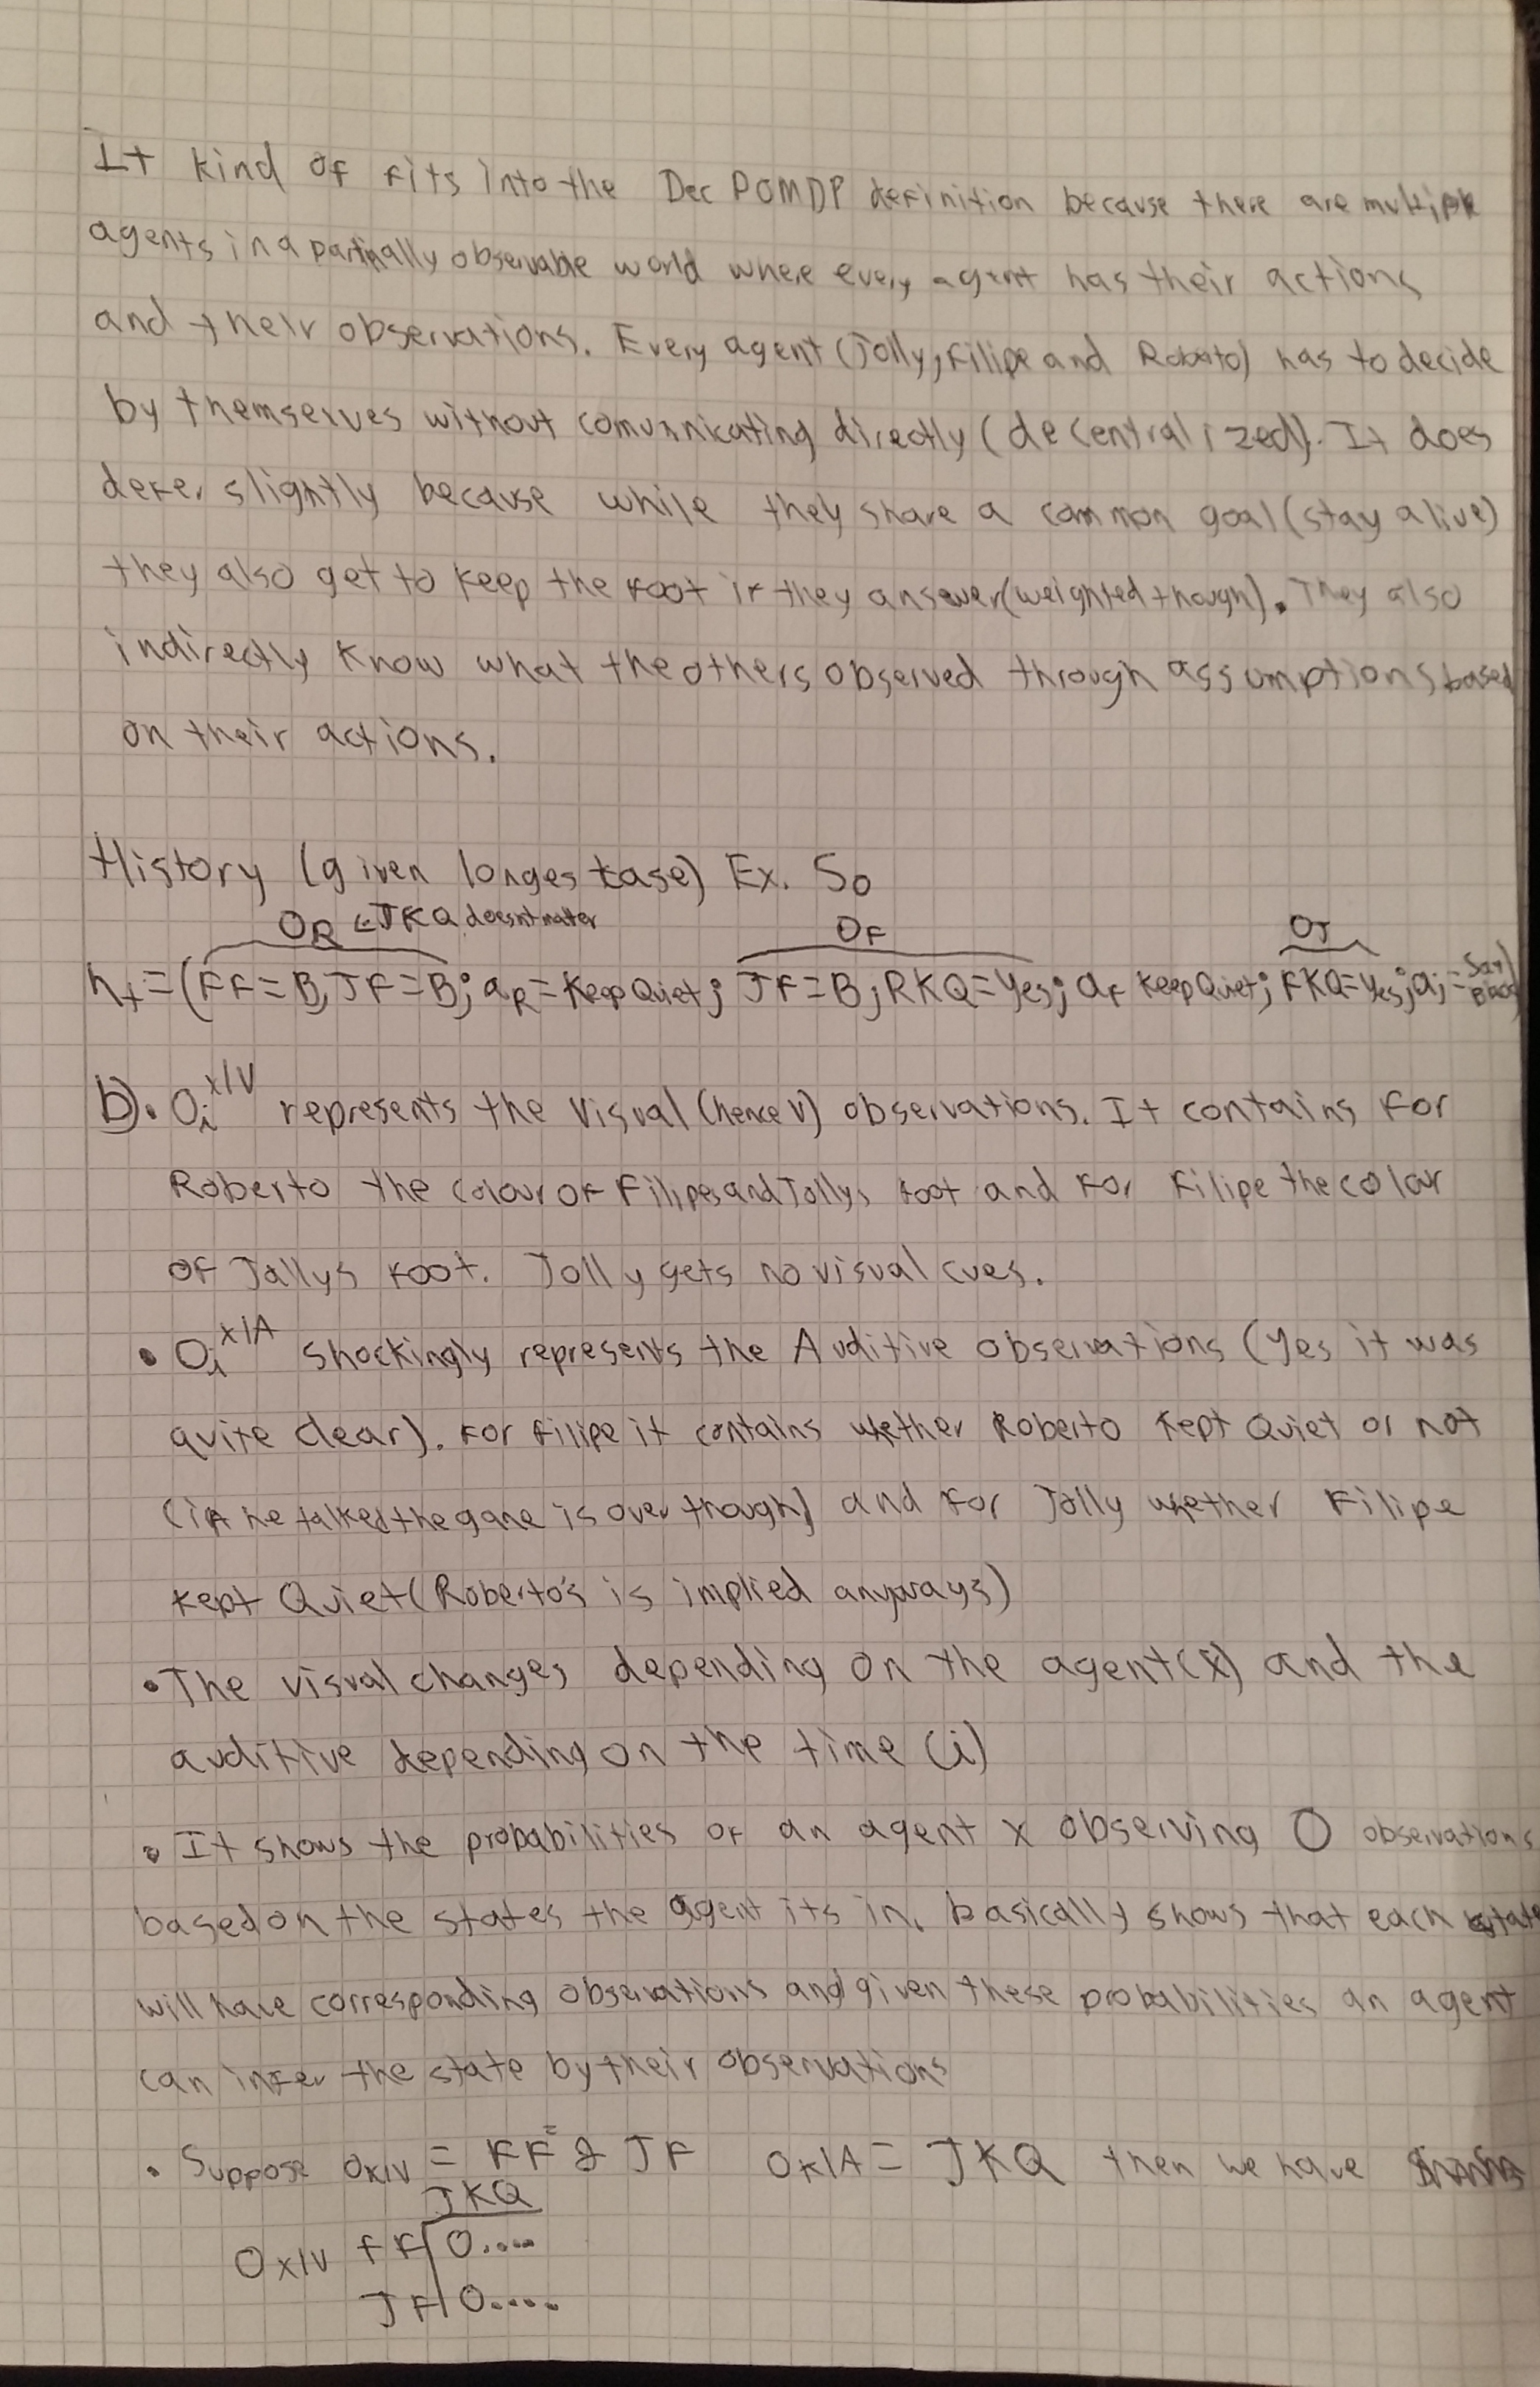
\includegraphics[scale=0.2]{p3.jpg}	
		\newpage

	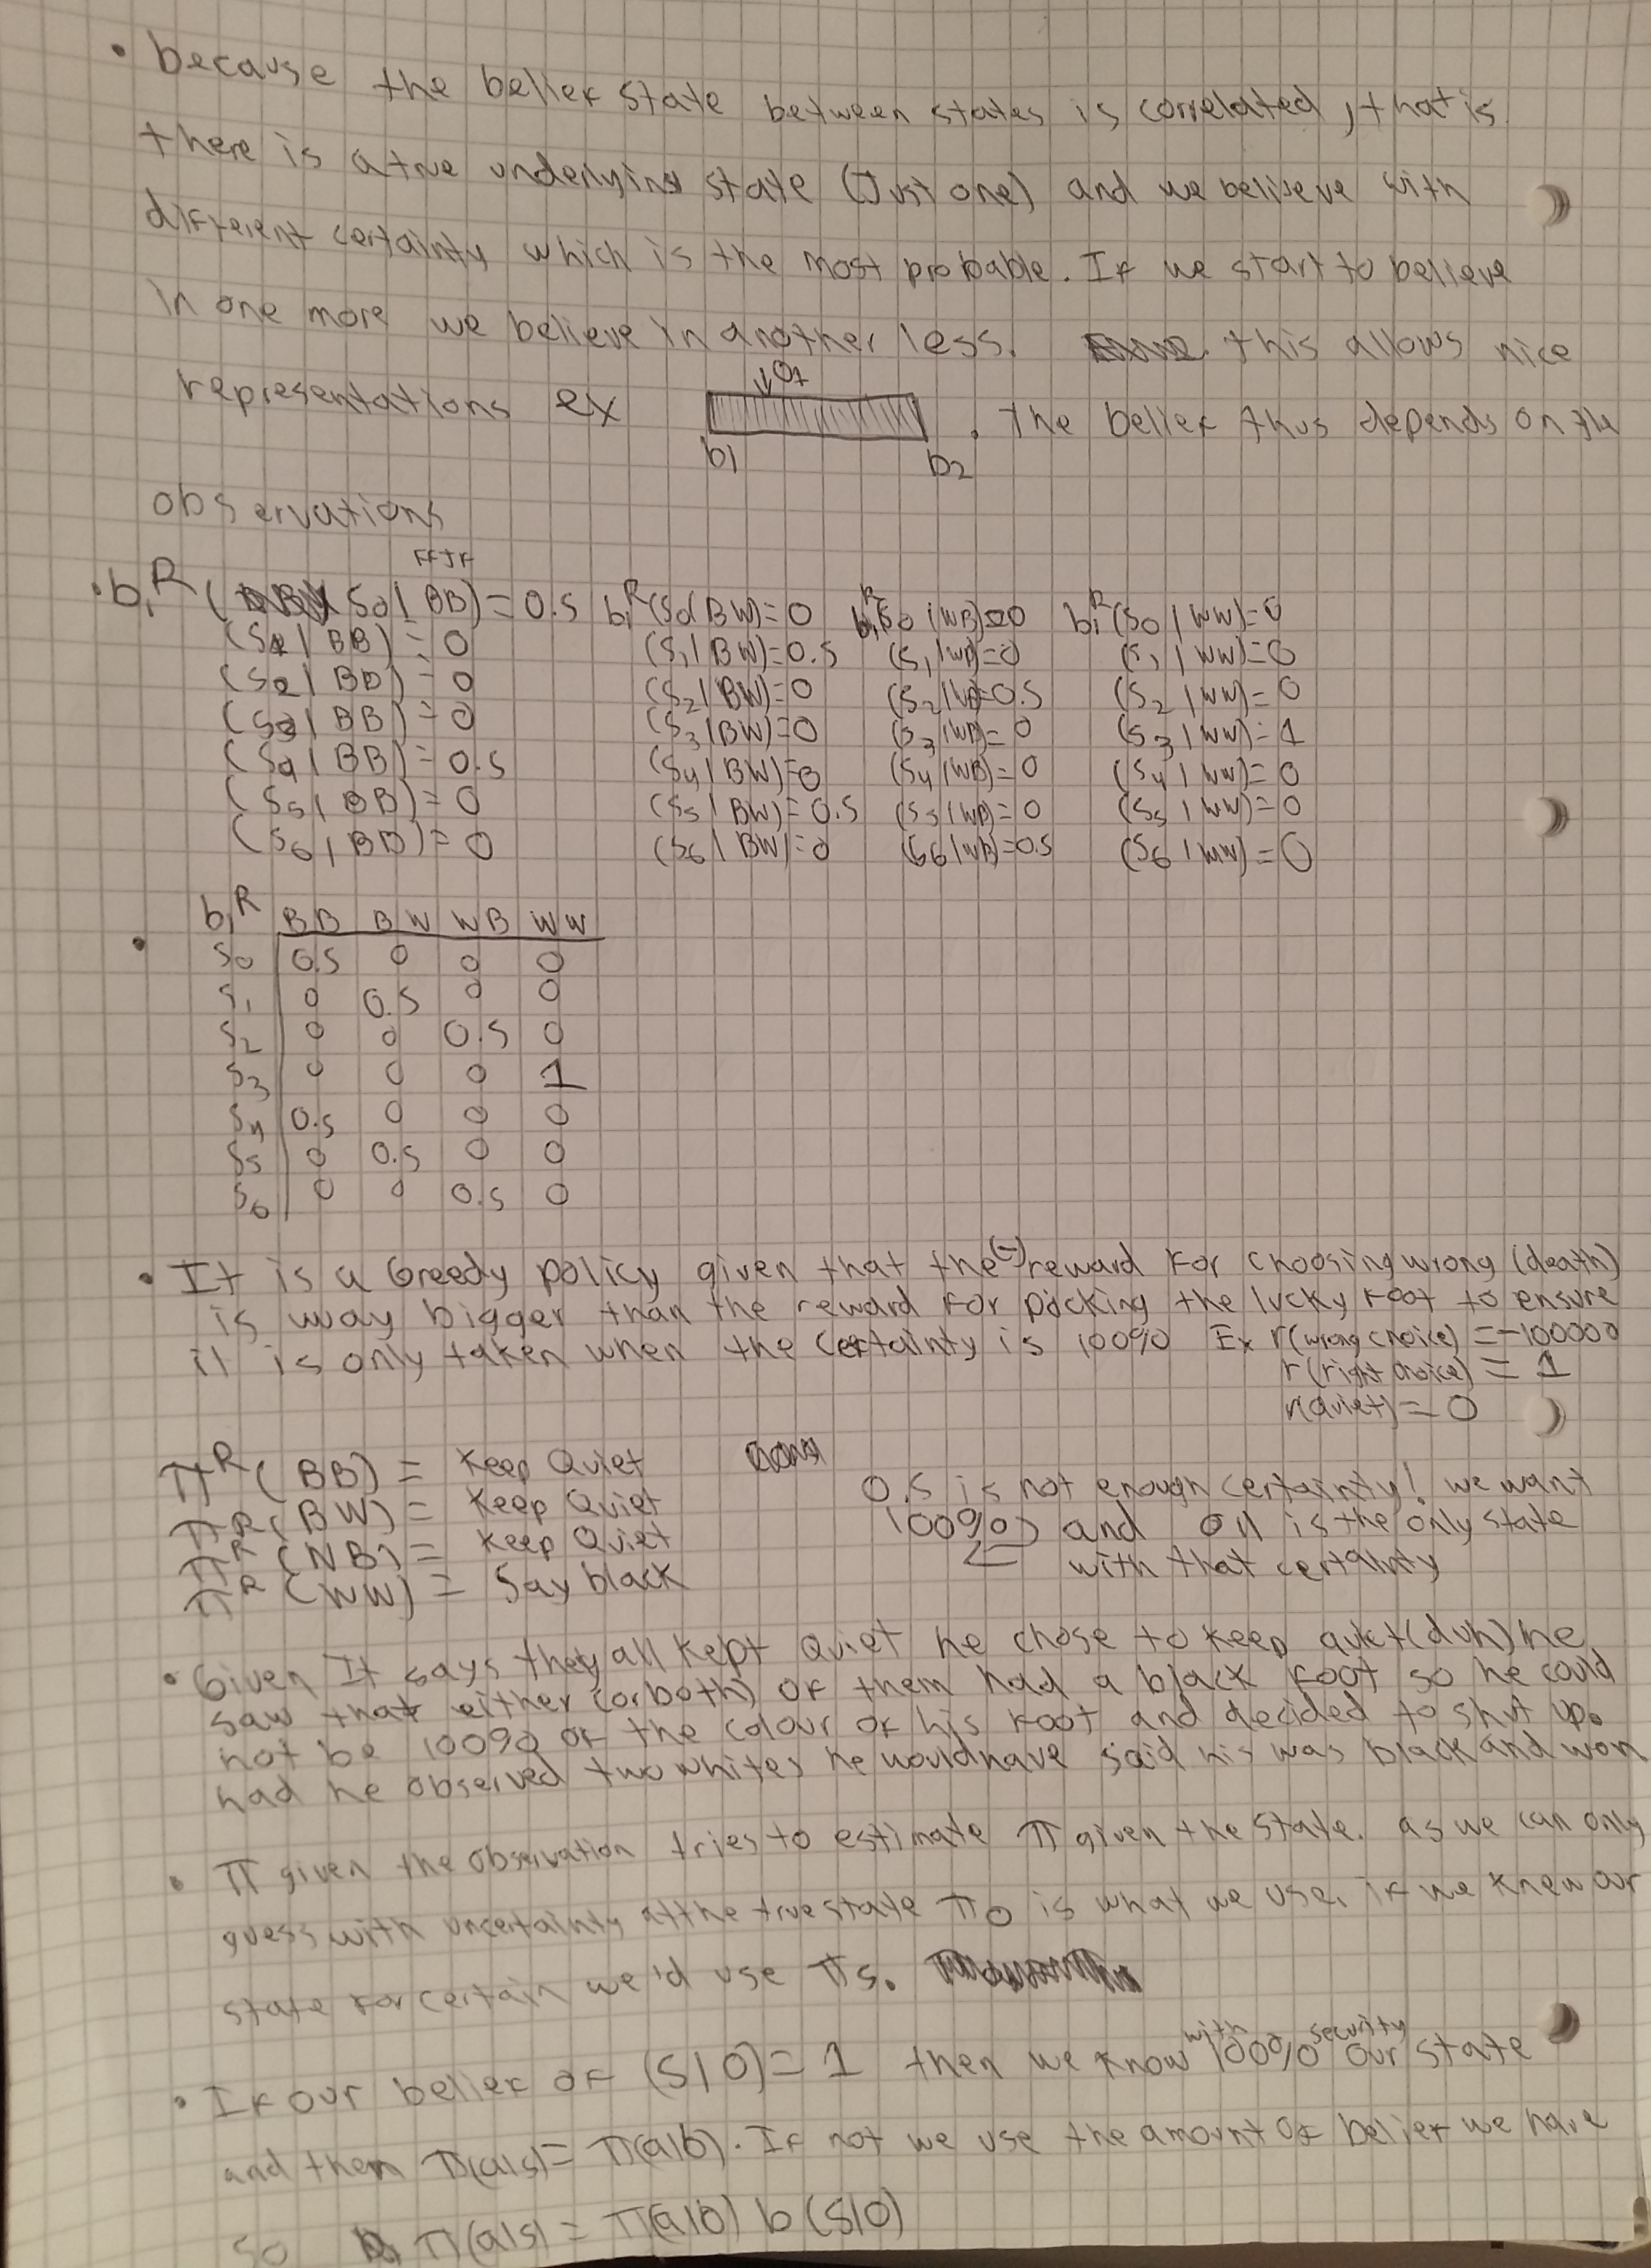
\includegraphics[scale=0.2]{p4.jpg}	
		\newpage

	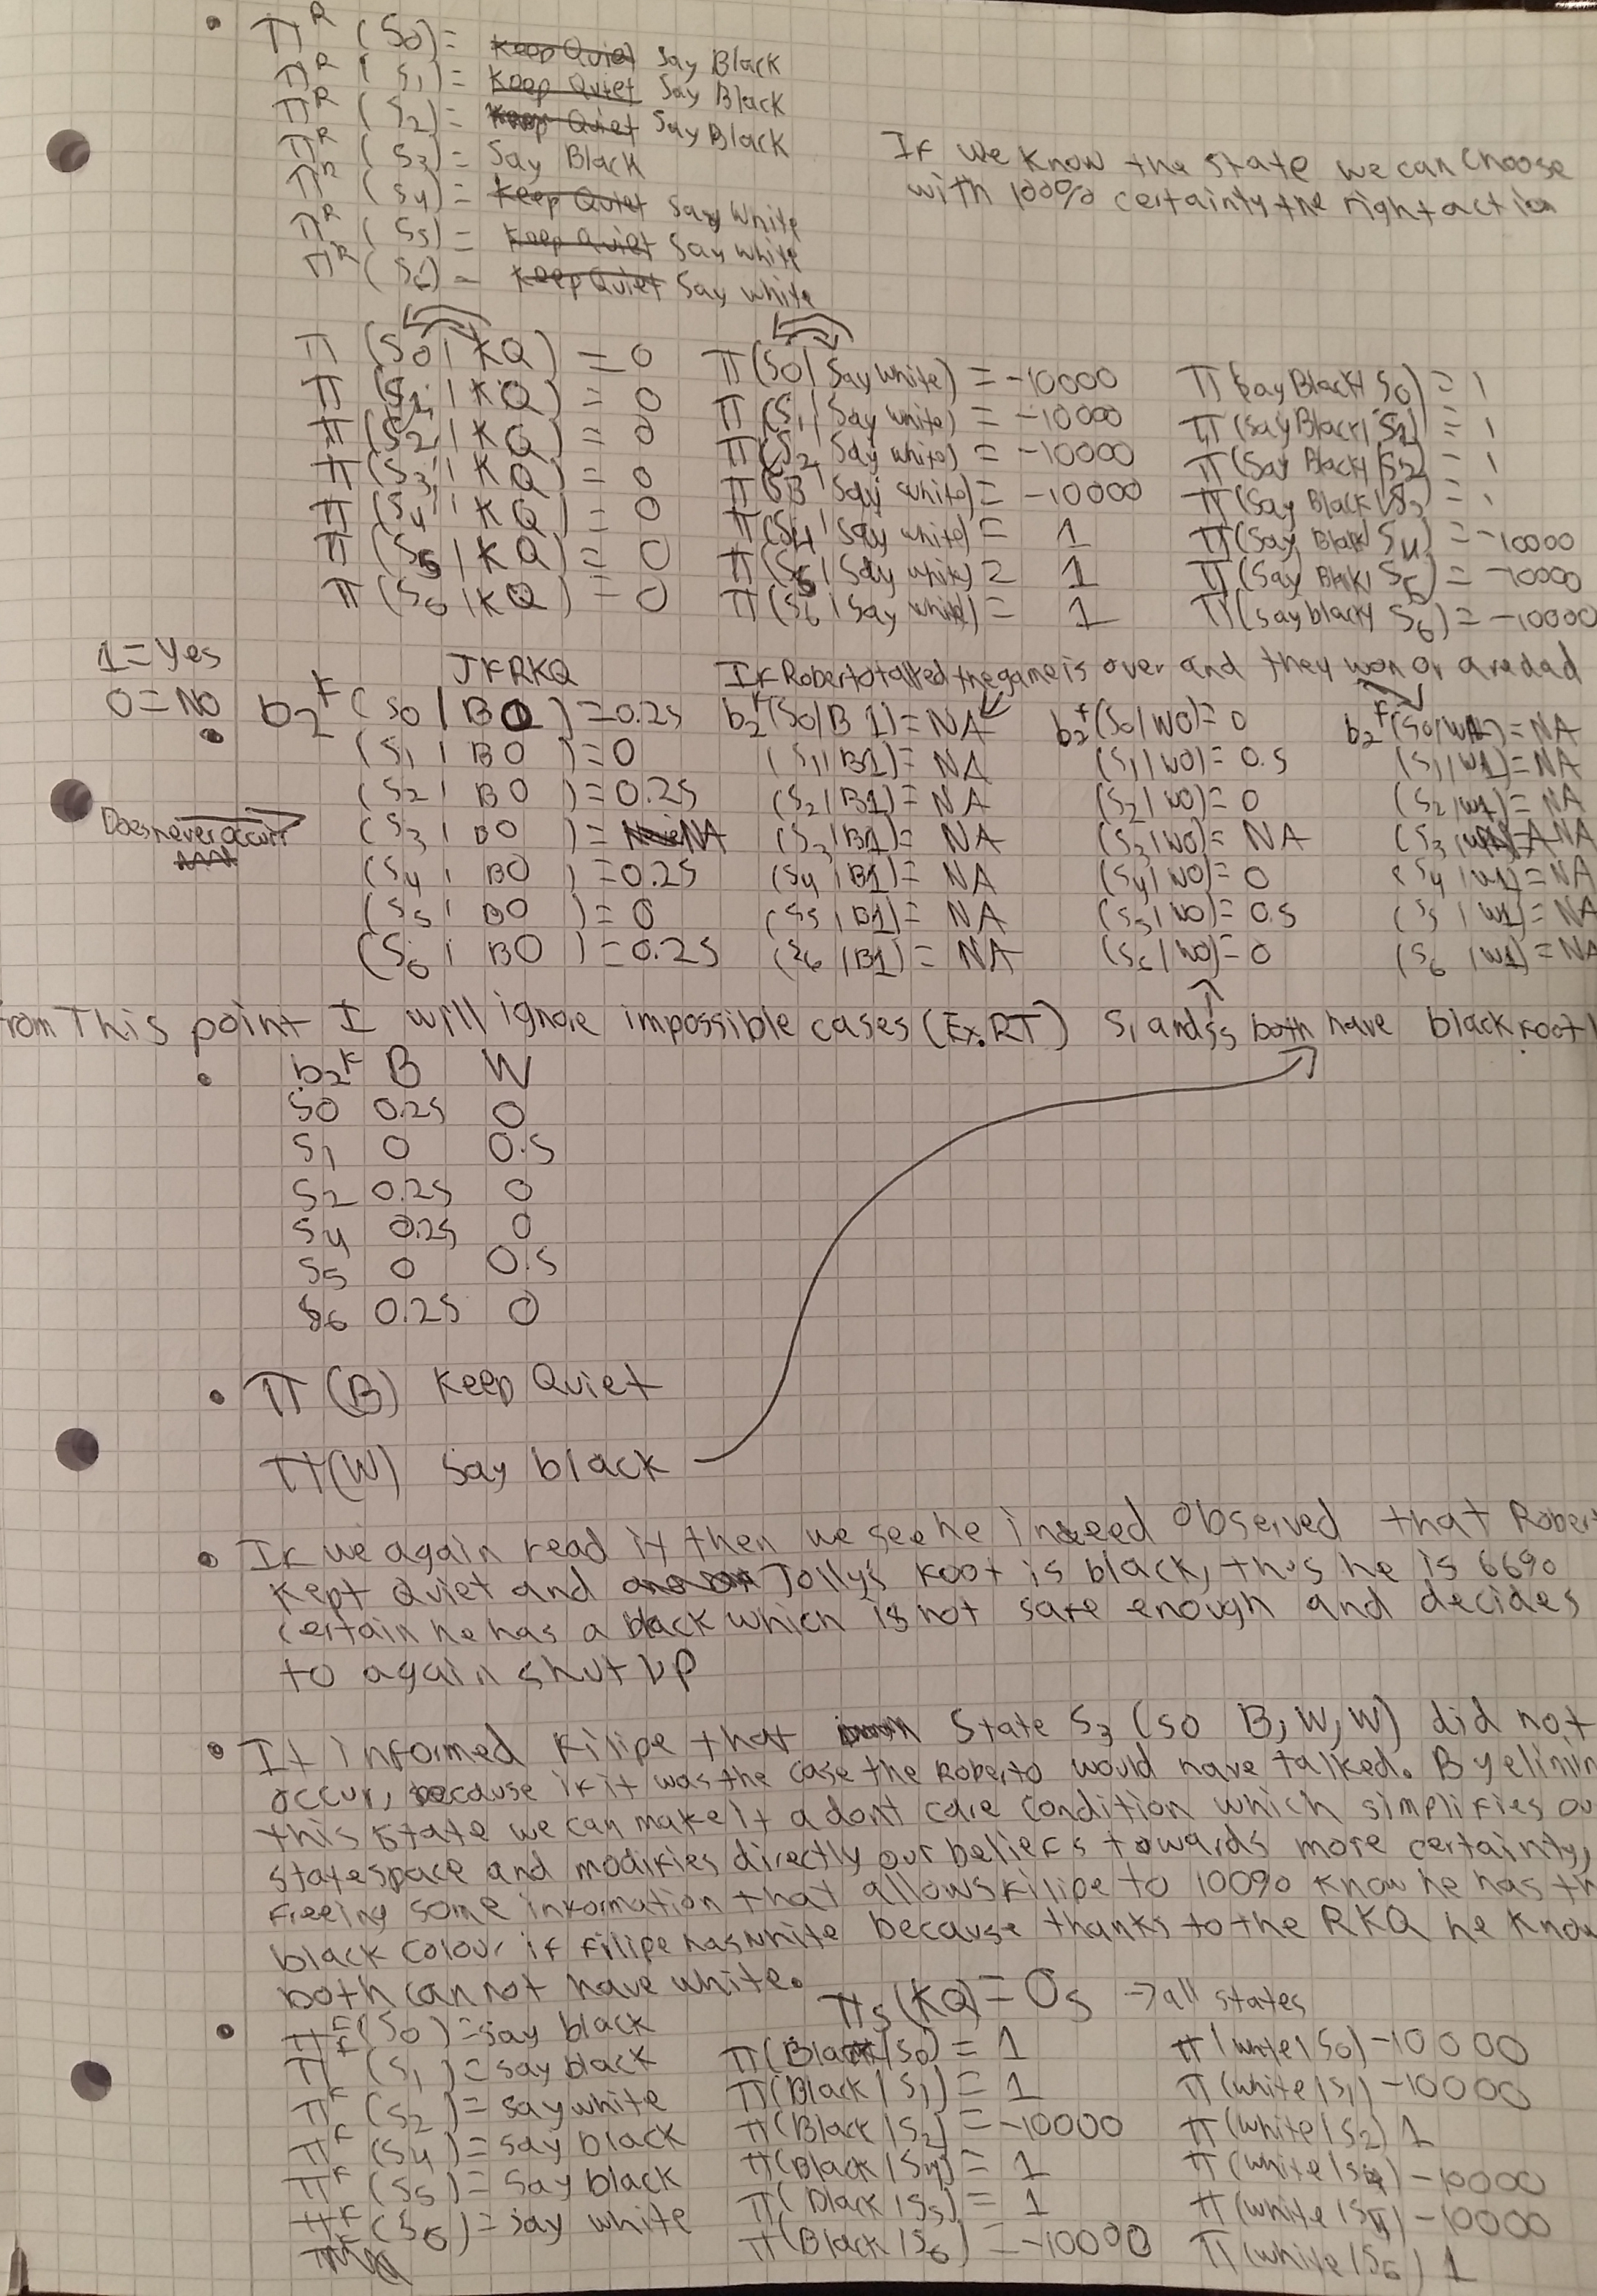
\includegraphics[scale=0.2]{p5.jpg}	
		\newpage

	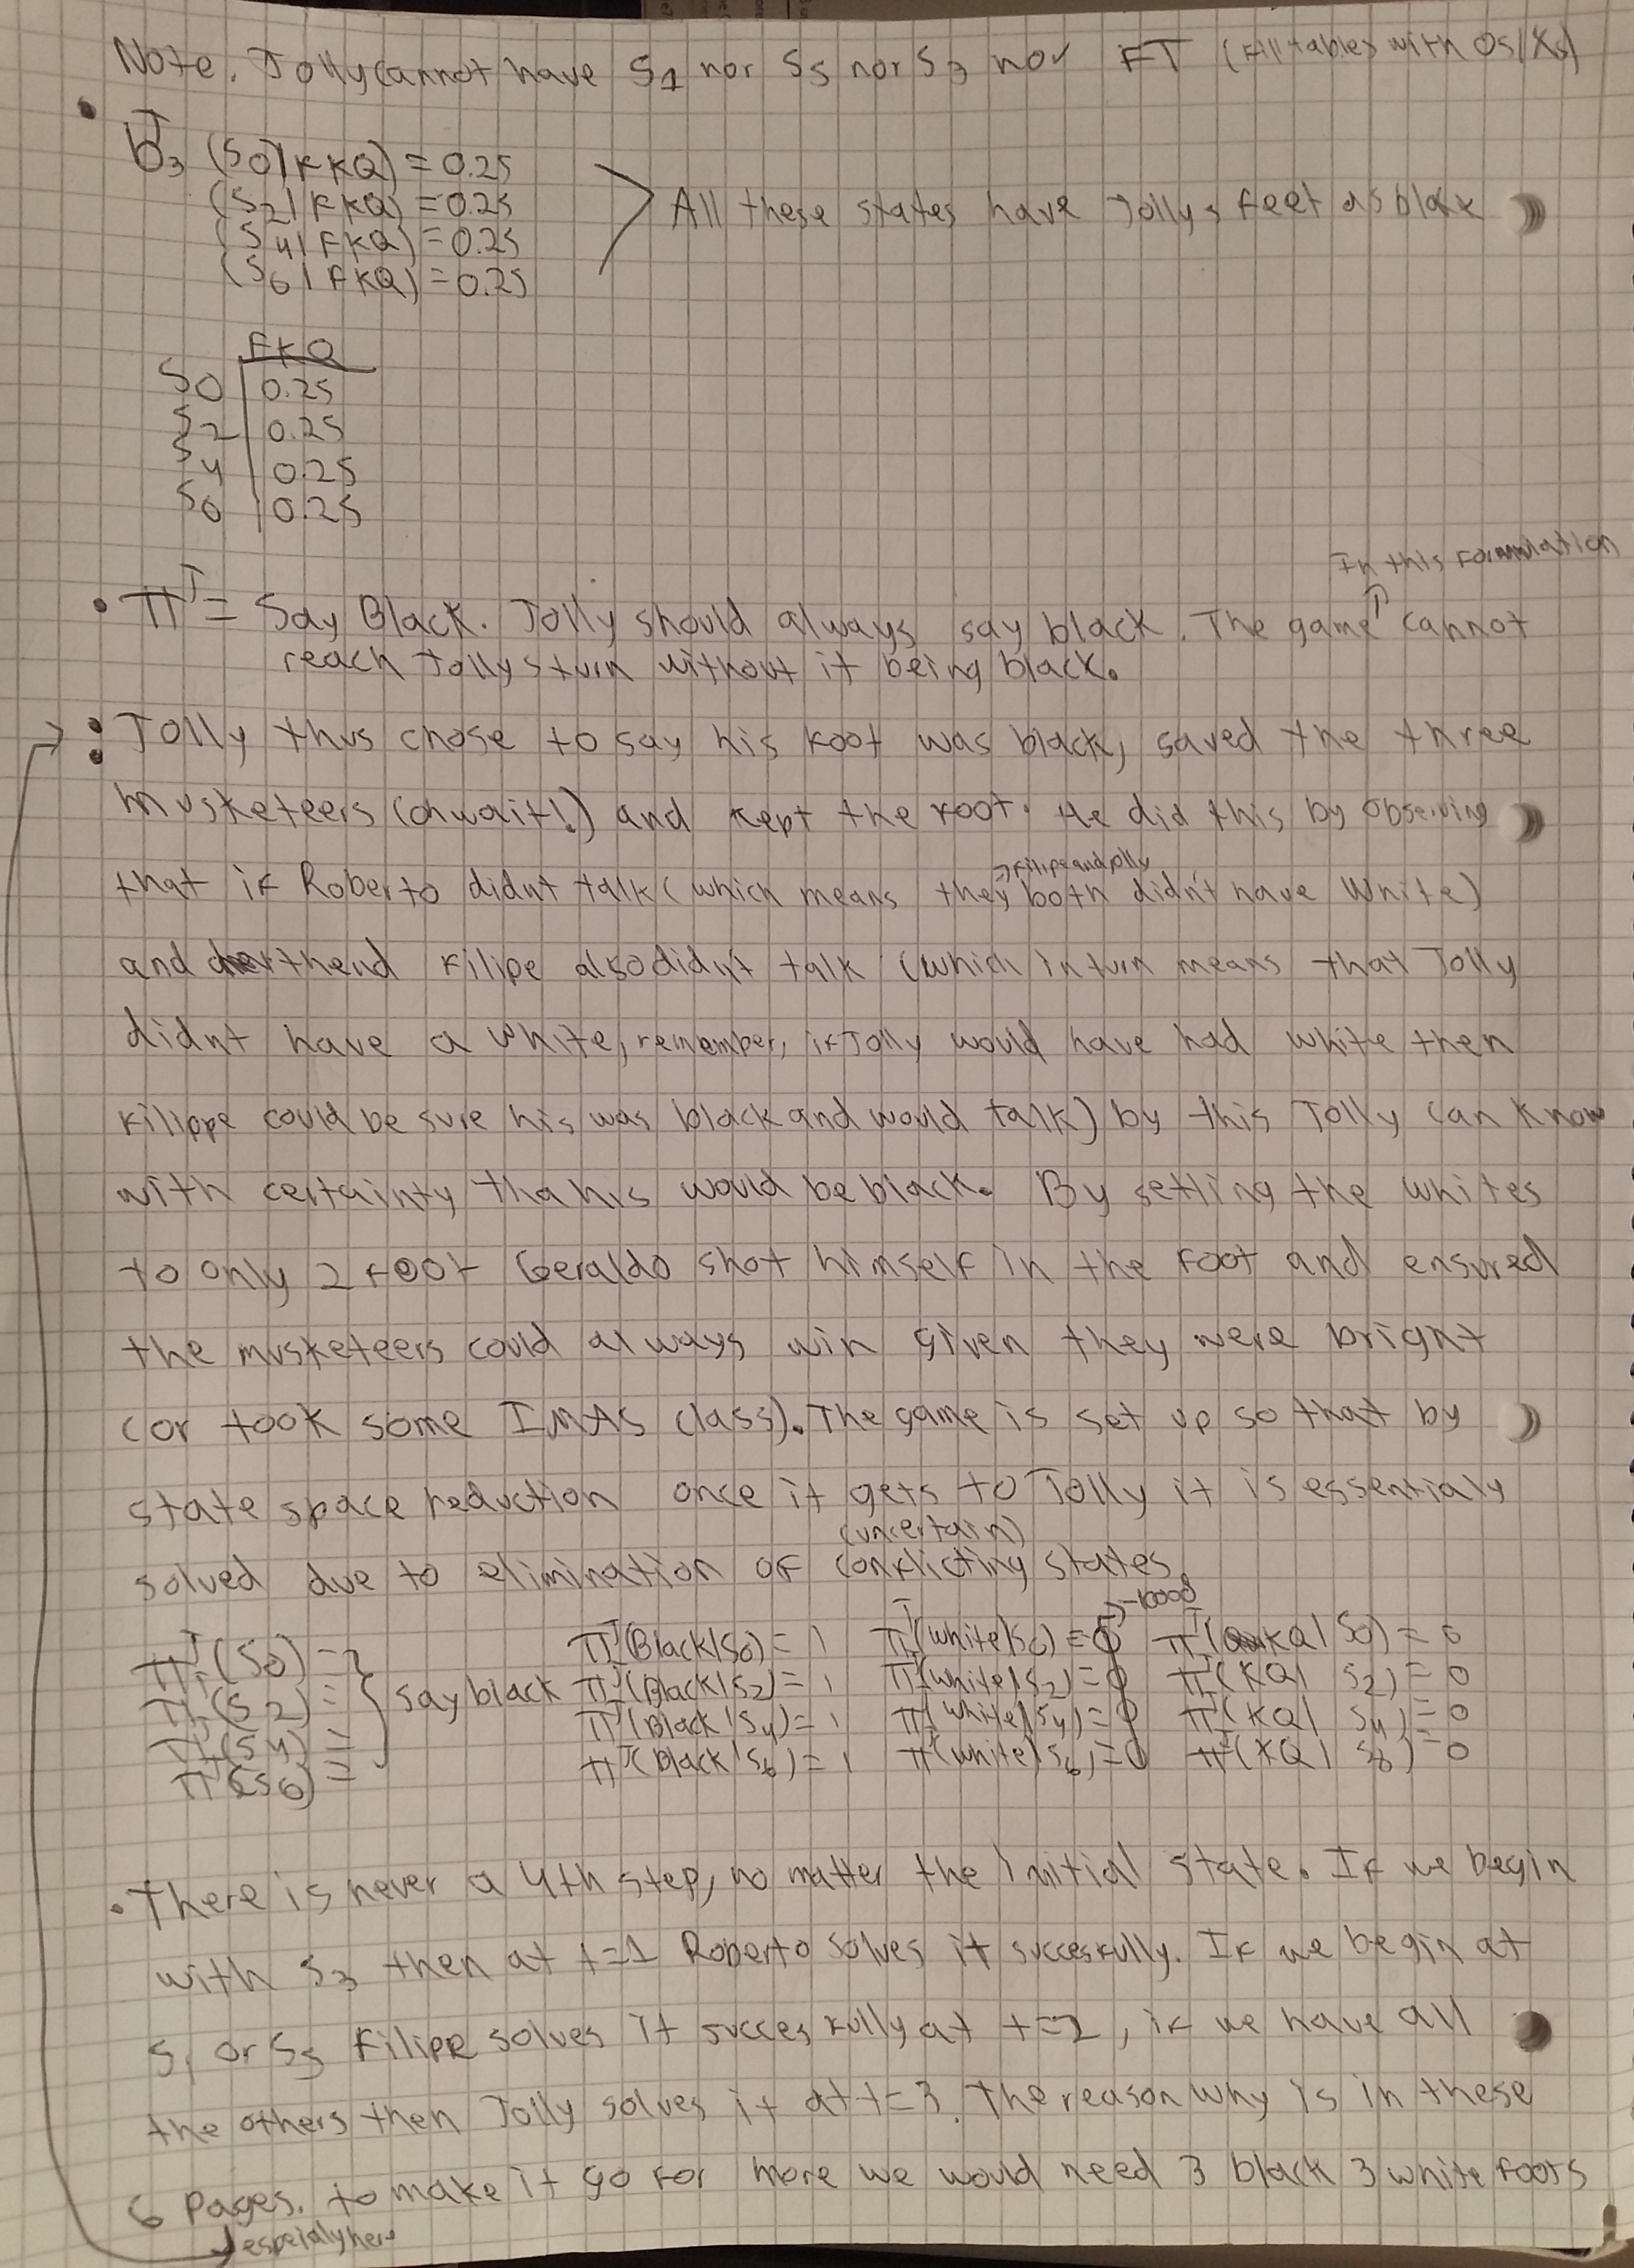
\includegraphics[scale=0.2]{p6.jpg}
		\newpage

\end{question}
%----------------------------------------------
\end{questions}



